\documentclass{beamer}
\usetheme{Madrid}
\usecolortheme{default}
\usepackage{tikz}
\usepackage{amsmath}
\usepackage{amssymb}

\title{Introduction to Categorical Logic}
\author{Brendan Shea, PhD}
\date{Introduction to Logic}

\begin{document}
	
	\begin{frame}
		\titlepage
	\end{frame}
	
	\begin{frame}{Categorical Logic: The Art of Valid Reasoning}
		\begin{itemize}
			\item \textbf{Categorical logic} is a system for analyzing and evaluating arguments based on relationships between categories or classes of objects.
			\item This logical system was first developed by Aristotle over 2,300 years ago and remains foundational to modern logical reasoning.
			\item Categorical logic focuses on determining whether an argument's conclusion necessarily follows from its premises.
			\item Understanding categorical logic helps us identify fallacies and construct valid arguments in everyday reasoning.
		\end{itemize}
		
		\begin{alertblock}{Why Study Categorical Logic?}
			Categorical logic provides a systematic framework for evaluating the validity of arguments without reference to their specific content, allowing us to focus on the form of reasoning itself.
		\end{alertblock}
	\end{frame}
	
	\begin{frame}{The Historical Foundations: Aristotle's Contribution}
		\begin{itemize}
			\item Aristotle introduced categorical logic in his work \textit{Prior Analytics} as part of his broader study of reasoning called the \textbf{Organon}.
			\item He identified that valid arguments must follow specific patterns or \textbf{syllogisms} that guarantee the truth of conclusions when premises are true.
			\item Aristotle's approach revolutionized thinking by separating the form of arguments from their content.
			\item This system remained the dominant framework for logical analysis for nearly two millennia.
		\end{itemize}
		
		\begin{center}
			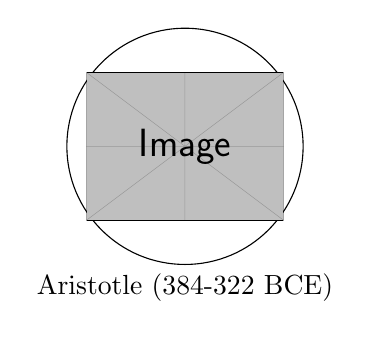
\begin{tikzpicture}
				\draw (0,0) circle (1.5cm);
				\node at (0,0) {\includegraphics[width=2.5cm]{example-image}};
				\node at (0,-1.8) {Aristotle (384-322 BCE)};
			\end{tikzpicture}
		\end{center}
	\end{frame}
	
	\begin{frame}{Deductive vs. Inductive Logic: Key Differences}
		\begin{itemize}
			\item \textbf{Deductive logic} (which includes categorical logic) moves from general principles to specific conclusions where the conclusion necessarily follows from the premises.
			\item \textbf{Inductive logic} moves from specific observations to general conclusions, establishing probability rather than certainty.
			\item Categorical logic is a form of deductive reasoning that guarantees valid conclusions when the argument follows correct form and has true premises.
			\item The certainty of deductive conclusions makes categorical logic particularly valuable for establishing definitive knowledge.
		\end{itemize}
		
		\begin{block}{Comparison of Logical Approaches}
			\scriptsize
			\begin{tabular}{|l|l|}
				\hline
				\textbf{Deductive Logic} & \textbf{Inductive Logic} \\
				\hline
				General to specific & Specific to general \\
				Certainty & Probability \\
				Truth-preserving & Strength of evidence \\
				Necessary conclusions & Likely conclusions \\
				\hline
			\end{tabular}
		\end{block}
	\end{frame}
	
	\begin{frame}{Why Categorical Logic Matters in Modern Thinking}
		\begin{itemize}
			\item Categorical logic provides a foundation for critical thinking that extends beyond academic philosophy.
			\item Understanding categorical reasoning helps us evaluate claims in science, law, politics, and everyday discourse.
			\item Many contemporary arguments can be analyzed using the principles of categorical logic, revealing their underlying structure.
			\item The ability to identify valid and invalid argument forms helps protect against manipulation through faulty reasoning.
		\end{itemize}
		
		\begin{example}
			A scientist argues: "All effective vaccines produce antibodies. This experimental treatment produces antibodies. Therefore, this experimental treatment is an effective vaccine."
			
			Using categorical logic, we can identify this as an invalid argument form, regardless of the truth of its premises.
		\end{example}
	\end{frame}
	
	\begin{frame}{The Four Types of Categorical Statements: A, E, I, O}
		\begin{itemize}
			\item Categorical logic analyzes arguments built from four standard types of statements about categories.
			\item Each type of statement has a specific \textbf{quality} (affirmative or negative) and \textbf{quantity} (universal or particular).
			\item The four types are traditionally labeled using the first four vowels: A, E, I, and O.
			\item Every categorical statement relates two terms: a \textbf{subject term} (S) and a \textbf{predicate term} (P).
		\end{itemize}
		
		\begin{block}{The Four Standard Forms}
			\begin{itemize}
				\item \textbf{A: Universal Affirmative} - "All S are P"
				\item \textbf{E: Universal Negative} - "No S are P"
				\item \textbf{I: Particular Affirmative} - "Some S are P"
				\item \textbf{O: Particular Negative} - "Some S are not P"
			\end{itemize}
		\end{block}
	\end{frame}
	
	\begin{frame}{Universal Affirmative (A): "All S are P"}
		\begin{itemize}
			\item An \textbf{A statement} claims that every member of the subject class is also a member of the predicate class.
			\item The form "All S are P" indicates that the entire subject class is included within the predicate class.
			\item A statements are \textbf{universal} in quantity (they refer to all members of the subject class) and \textbf{affirmative} in quality.
			\item In categorical logic, "All S are P" means exactly the same as "Every S is P."
		\end{itemize}
		
		\begin{center}
			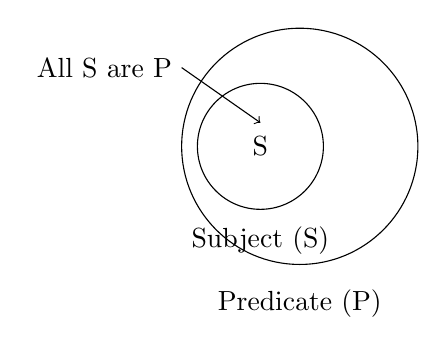
\begin{tikzpicture}
				\draw (0,0) circle (1.5cm) node[below=1.7cm] {Predicate (P)};
				\draw (-0.5,0) circle (0.8cm) node[below=0.9cm] {Subject (S)};
				\node at (-0.5,0) {S};
				\draw[->] (-1.5,1) node[left] {All S are P} to (-0.5,0.3);
			\end{tikzpicture}
		\end{center}
	\end{frame}
	
	\begin{frame}{Universal Negative (E): "No S are P"}
		\begin{itemize}
			\item An \textbf{E statement} claims that no member of the subject class is a member of the predicate class.
			\item The form "No S are P" indicates that the subject class and predicate class are completely separate.
			\item E statements are \textbf{universal} in quantity (they refer to all members of the subject class) and \textbf{negative} in quality.
			\item Logically, "No S are P" means the same as "No P are S" - both indicate mutual exclusion of the categories.
		\end{itemize}
		
		\begin{center}
			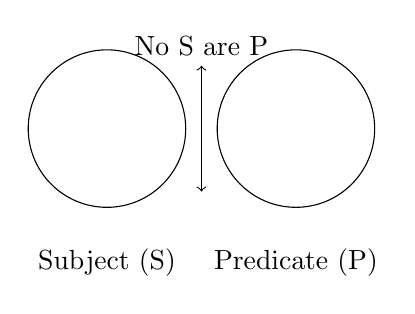
\begin{tikzpicture}
				\draw (1.2,0) circle (1.0cm) node[below=1.4cm] {Predicate (P)};
				\draw (-1.2,0) circle (1.0cm) node[below=1.4cm] {Subject (S)};
				\draw[<->] (0,0.8) node[above] {No S are P} to (0,-0.8);
			\end{tikzpicture}
		\end{center}
	\end{frame}
	
	\begin{frame}{Particular Affirmative (I): "Some S are P"}
		\begin{itemize}
			\item An \textbf{I statement} claims that at least one member of the subject class is also a member of the predicate class.
			\item The form "Some S are P" indicates that there is at least partial overlap between the subject and predicate classes.
			\item I statements are \textbf{particular} in quantity (they refer to at least one, but not necessarily all, members of the subject class) and \textbf{affirmative} in quality.
			\item In logic, "some" means "at least one" and possibly all, not "only some" as in everyday speech.
		\end{itemize}
		
		\begin{center}
			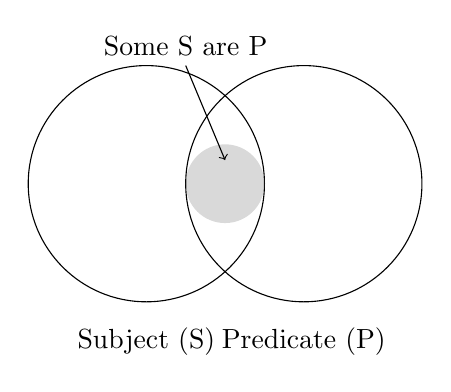
\begin{tikzpicture}
				\draw (1,0) circle (1.5cm) node[below=1.7cm] {Predicate (P)};
				\draw (-1,0) circle (1.5cm) node[below=1.7cm] {Subject (S)};
				\fill[gray, opacity=0.3] (0,0) circle (0.5cm);
				\draw[->] (-0.5,1.5) node[above] {Some S are P} to (0,0.3);
			\end{tikzpicture}
		\end{center}
	\end{frame}
	
	\begin{frame}{Particular Negative (O): "Some S are not P"}
		\begin{itemize}
			\item An \textbf{O statement} claims that at least one member of the subject class is not a member of the predicate class.
			\item The form "Some S are not P" indicates that the subject class is not completely contained within the predicate class.
			\item O statements are \textbf{particular} in quantity (they refer to at least one, but not necessarily all, members of the subject class) and \textbf{negative} in quality.
			\item O statements are compatible with situations where most, but not all, S are P.
		\end{itemize}
		
		\begin{center}
			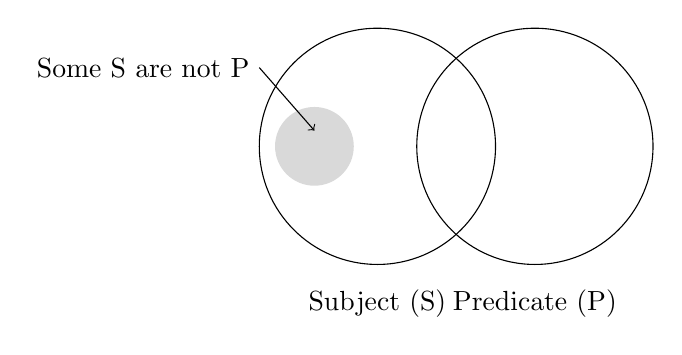
\begin{tikzpicture}
				\draw (1,0) circle (1.5cm) node[below=1.7cm] {Predicate (P)};
				\draw (-1,0) circle (1.5cm) node[below=1.7cm] {Subject (S)};
				\fill[gray, opacity=0.3] (-1.8,0) circle (0.5cm);
				\draw[->] (-2.5,1) node[left] {Some S are not P} to (-1.8,0.2);
			\end{tikzpicture}
		\end{center}
	\end{frame}
	
	\begin{frame}{The Square of Opposition: Relationships Between Statement Types}
		\begin{itemize}
			\item The \textbf{Square of Opposition} illustrates the logical relationships between the four types of categorical statements.
			\item \textbf{Contradictory} statements cannot both be true or both be false (A and O; E and I).
			\item \textbf{Contrary} statements cannot both be true but both can be false (A and E).
			\item \textbf{Subcontrary} statements cannot both be false but both can be true (I and O).
		\end{itemize}
		
		\begin{center}
			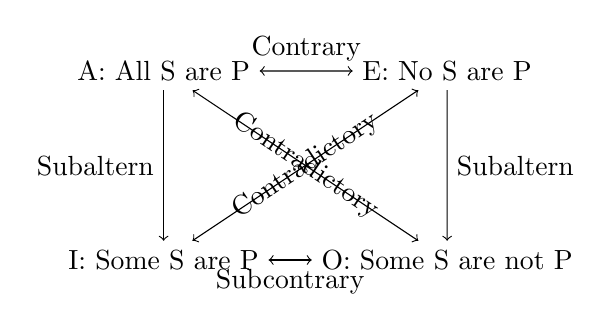
\begin{tikzpicture}[scale=1.2]
				\node (A) at (0,2) {A: All S are P};
				\node (E) at (3,2) {E: No S are P};
				\node (I) at (0,0) {I: Some S are P};
				\node (O) at (3,0) {O: Some S are not P};
				
				\draw[<->] (A) -- (E) node[midway, above] {Contrary};
				\draw[<->] (I) -- (O) node[midway, below] {Subcontrary};
				\draw[<->] (A) -- (O) node[midway, sloped] {Contradictory};
				\draw[<->] (E) -- (I) node[midway, sloped] {Contradictory};
				\draw[->] (A) -- (I) node[midway, left] {Subaltern};
				\draw[->] (E) -- (O) node[midway, right] {Subaltern};
			\end{tikzpicture}
		\end{center}
	\end{frame}
	
	\begin{frame}{Example: Analyzing Everyday Statements Using the A, E, I, O Framework}
		\begin{itemize}
			\item Everyday claims can be translated into standard categorical form to analyze their logical relationships.
			\item Identifying the correct categorical form helps reveal hidden assumptions and implications.
			\item Some statements that appear different in natural language are logically equivalent in categorical form.
			\item Complex statements may need to be broken down into multiple categorical statements.
		\end{itemize}
		
		\begin{block}{Examples of Translation}
			\scriptsize
			\begin{itemize}
				\item "Dogs are mammals" $\rightarrow$ A: All dogs are mammals
				\item "No politicians are trustworthy" $\rightarrow$ E: No politicians are trustworthy people
				\item "Some students passed the exam" $\rightarrow$ I: Some students are exam-passers
				\item "Not every computer is reliable" $\rightarrow$ O: Some computers are not reliable devices
			\end{itemize}
		\end{block}
	\end{frame}
	
	\begin{frame}{What is a Categorical Syllogism? Basic Structure}
		\begin{itemize}
			\item A \textbf{categorical syllogism} is a deductive argument consisting of exactly three categorical statements: two premises and one conclusion.
			\item Each categorical syllogism contains exactly three terms, with each term appearing exactly twice in the argument.
			\item The premises establish a relationship between terms that, if the syllogism is valid, necessitates the conclusion.
			\item The fundamental principle of syllogistic reasoning is that things that share a common property are related to each other in specific ways.
		\end{itemize}
		
		\begin{example}
			Premise 1: All mammals are warm-blooded animals.\\
			Premise 2: All dogs are mammals.\\
			Conclusion: Therefore, all dogs are warm-blooded animals.
		\end{example}
	\end{frame}
	
	\begin{frame}{The Three Terms: Major, Minor, and Middle}
		\begin{itemize}
			\item Every categorical syllogism contains exactly three terms, each serving a specific function in the argument.
			\item The \textbf{major term} (P) appears in the conclusion as the predicate and tells us what is being claimed about the subject.
			\item The \textbf{minor term} (S) appears in the conclusion as the subject and represents what the argument is primarily about.
			\item The \textbf{middle term} (M) appears once in each premise but not in the conclusion, connecting the major and minor terms.
		\end{itemize}
		
		\begin{center}
			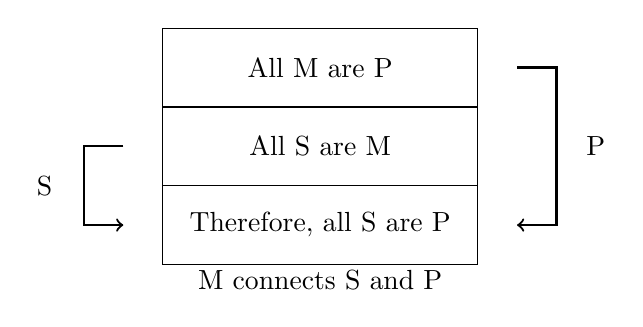
\begin{tikzpicture}
				\node[draw, rectangle, minimum width=4cm, minimum height=1cm] at (0,2) {All M are P};
				\node[draw, rectangle, minimum width=4cm, minimum height=1cm] at (0,1) {All S are M};
				\node[draw, rectangle, minimum width=4cm, minimum height=1cm] at (0,0) {Therefore, all S are P};
				\draw[->, thick] (2.5,2) -- (3,2) -- (3,0) -- (2.5,0);
				\draw[->, thick] (-2.5,1) -- (-3,1) -- (-3,0) -- (-2.5,0);
				\node at (-3.5,0.5) {S};
				\node at (3.5,1) {P};
				\node at (0,-0.7) {M connects S and P};
			\end{tikzpicture}
		\end{center}
	\end{frame}
	
	\begin{frame}{Major and Minor Premises: Building the Argument}
		\begin{itemize}
			\item The \textbf{major premise} contains the major term (P) and the middle term (M), establishing how the predicate of the conclusion relates to the middle term.
			\item The \textbf{minor premise} contains the minor term (S) and the middle term (M), establishing how the subject of the conclusion relates to the middle term.
			\item The arrangement of these premises creates a chain of reasoning that leads to the conclusion.
			\item The ordering of premises in presentation does not affect the validity of the syllogism, though standard form puts the major premise first.
		\end{itemize}
		
		\begin{alertblock}{Important Note}
			The middle term (M) must be used to establish a clear relationship between the major and minor terms. If the middle term fails to properly connect them, the syllogism will be invalid regardless of whether its premises are true.
		\end{alertblock}
	\end{frame}
	
	\begin{frame}{Distribution of Terms in Categorical Statements}
		\begin{itemize}
			\item A term is \textbf{distributed} in a statement when the statement refers to all members of the class designated by that term.
			\item Understanding distribution is crucial for determining the validity of syllogisms.
			\item In A statements ("All S are P"), the subject term is distributed, but the predicate term is undistributed.
			\item In E statements ("No S are P"), both the subject and predicate terms are distributed.
		\end{itemize}
		
		\begin{block}{Distribution Rules}
			\begin{tabular}{|l|l|l|}
				\hline
				\textbf{Statement Type} & \textbf{Subject} & \textbf{Predicate} \\
				\hline
				A: All S are P & Distributed & Undistributed \\
				E: No S are P & Distributed & Distributed \\
				I: Some S are P & Undistributed & Undistributed \\
				O: Some S are not P & Undistributed & Distributed \\
				\hline
			\end{tabular}
		\end{block}
	\end{frame}
	
	\begin{frame}{Example: Breaking Down a Valid Categorical Syllogism}
		\begin{itemize}
			\item Let's analyze a valid categorical syllogism step by step to understand how it works.
			\item We'll identify the three terms and check if the middle term successfully connects the minor and major terms.
			\item We'll examine the distribution of terms to verify that the syllogism follows the rules of validity.
			\item This analysis will demonstrate why the conclusion necessarily follows from the premises.
		\end{itemize}
		
		\begin{example}
			\scriptsize
			Premise 1: All philosophers are critical thinkers. (A)\\
			Premise 2: Socrates is a philosopher. (A)\\
			Conclusion: Therefore, Socrates is a critical thinker. (A)\\
			
			\textbf{Terms:} Minor (S): Socrates; Middle (M): philosopher; Major (P): critical thinker\\
			\textbf{Analysis:} Middle term connects S and P and is properly distributed in premise 2.
		\end{example}
	\end{frame}
	
	\begin{frame}{Example: Identifying Flaws in Invalid Syllogisms}
		\begin{itemize}
			\item Invalid syllogisms fail to establish a necessary connection between the premises and conclusion.
			\item Common flaws include undistributed middle terms, illicit processes, and negative premise problems.
			\item Recognizing these patterns helps identify faulty reasoning in everyday arguments.
			\item An argument can have true premises and a true conclusion but still be invalid if the conclusion doesn't necessarily follow from the premises.
		\end{itemize}
		
		\begin{alertblock}{Invalid Syllogism Example}
			Premise 1: All dogs are mammals. (A)\\
			Premise 2: All cats are mammals. (A)\\
			Conclusion: Therefore, all dogs are cats. (A)\\
			
			\textbf{Flaw:} Undistributed middle term. "Mammals" appears as a predicate in both premises and is therefore undistributed, failing to establish a necessary connection between dogs and cats.
		\end{alertblock}
	\end{frame}
	
	\begin{frame}{Standard Form: Arranging Syllogisms for Analysis}
		\begin{itemize}
			\item A categorical syllogism in \textbf{standard form} follows specific conventions that make analysis easier.
			\item The major premise (containing the major term) is stated first, followed by the minor premise (containing the minor term).
			\item The conclusion is preceded by a marker like "therefore" or "thus" and contains the minor term as subject and major term as predicate.
			\item Converting arguments to standard form helps reveal their underlying logical structure and facilitates validity assessment.
		\end{itemize}
		
		\begin{block}{Standard Form Requirements}
			\begin{enumerate}
				\item Each statement must be in standard A, E, I, or O form
				\item The major premise (containing P) comes first
				\item The minor premise (containing S) comes second
				\item The conclusion has S as subject and P as predicate
				\item The middle term (M) appears in both premises but not the conclusion
			\end{enumerate}
		\end{block}
	\end{frame}
	
	\begin{frame}{Mood: The Pattern of A, E, I, O Statements}
		\begin{itemize}
			\item The \textbf{mood} of a syllogism is determined by the types of categorical statements (A, E, I, O) used in the argument.
			\item Mood is represented by three letters indicating the statement types of the major premise, minor premise, and conclusion, in that order.
			\item For example, an AAA syllogism has A statements (universal affirmatives) for both premises and the conclusion.
			\item Of the 64 possible moods, only a subset yield valid syllogisms.
		\end{itemize}
		
		\begin{center}
			\begin{tabular}{|l|l|}
				\hline
				\textbf{Mood} & \textbf{Example} \\
				\hline
				AAA & All M are P, All S are M, Therefore all S are P \\
				EIO & No M are P, Some S are M, Therefore some S are not P \\
				AII & All M are P, Some S are M, Therefore some S are P \\
				AOO & All M are P, Some S are not M, Therefore some S are not P \\
				\hline
			\end{tabular}
		\end{center}
	\end{frame}
	
	\begin{frame}{Figure: The Position of the Middle Term}
		\begin{itemize}
			\item The \textbf{figure} of a syllogism refers to the position of the middle term (M) in the premises.
			\item There are exactly four possible figures based on whether M appears as subject or predicate in each premise.
			\item The figure affects which moods can yield valid arguments, as certain arrangements facilitate valid reasoning while others do not.
			\item Together, mood and figure completely describe the form of a categorical syllogism.
		\end{itemize}
		
		\begin{center}
			\begin{tabular}{|c|c|c|c|}
				\hline
				\textbf{Figure 1} & \textbf{Figure 2} & \textbf{Figure 3} & \textbf{Figure 4} \\
				\hline
				M-P & P-M & M-P & P-M \\
				S-M & S-M & M-S & M-S \\
				S-P & S-P & S-P & S-P \\
				\hline
			\end{tabular}
		\end{center}
	\end{frame}
	
	\begin{frame}{The Four Figures of Syllogisms}
		\begin{itemize}
			\item \textbf{First Figure:} Middle term is subject in major premise and predicate in minor premise (M-P, S-M).
			\item \textbf{Second Figure:} Middle term is predicate in both premises (P-M, S-M).
			\item \textbf{Third Figure:} Middle term is subject in both premises (M-P, M-S).
			\item \textbf{Fourth Figure:} Middle term is predicate in major premise and subject in minor premise (P-M, M-S).
		\end{itemize}
		
		\begin{center}
			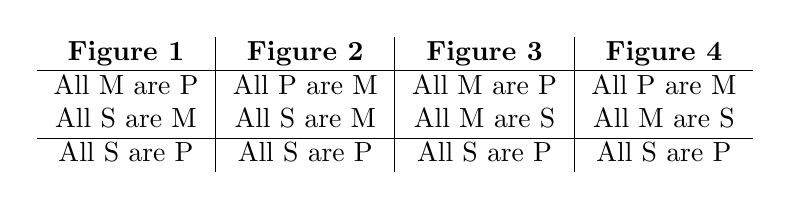
\begin{tikzpicture}
				\node at (0,0) {
					\begin{tabular}{c|c|c|c}
						\textbf{Figure 1} & \textbf{Figure 2} & \textbf{Figure 3} & \textbf{Figure 4} \\
						\hline
						All M are P & All P are M & All M are P & All P are M \\
						All S are M & All S are M & All M are S & All M are S \\
						\hline
						All S are P & All S are P & All S are P & All S are P
					\end{tabular}
				};
			\end{tikzpicture}
		\end{center}
	\end{frame}
	
	\begin{frame}{256 Possible Syllogistic Forms - But How Many Are Valid?}
		\begin{itemize}
			\item With 4 statement types (A, E, I, O), there are $4^3 = 64$ possible moods.
			\item Combined with 4 possible figures, there are $64 \times 4 = 256$ possible syllogistic forms.
			\item Of these 256 forms, only 24 are valid, representing 15 distinct argument patterns (some valid in multiple figures).
			\item Traditionally, valid forms were given mnemonic names like "Barbara" (AAA-1) and "Celarent" (EAE-1) to help students remember them.
		\end{itemize}
		
		\begin{block}{Some Valid Syllogism Forms}
			\scriptsize
			\begin{tabular}{|l|l|l|}
				\hline
				\textbf{Name} & \textbf{Mood-Figure} & \textbf{Example} \\
				\hline
				Barbara & AAA-1 & All M are P, All S are M, Therefore all S are P \\
				Celarent & EAE-1 & No M are P, All S are M, Therefore no S are P \\
				Darii & AII-1 & All M are P, Some S are M, Therefore some S are P \\
				Ferio & EIO-1 & No M are P, Some S are M, Therefore some S are not P \\
				\hline
			\end{tabular}
		\end{block}
	\end{frame}
	
	\begin{frame}{Example: Converting Arguments to Standard Form}
		\begin{itemize}
			\item Many everyday arguments are not presented in standard categorical form but can be translated for analysis.
			\item Converting to standard form involves identifying the three terms and restructuring the statements as A, E, I, or O.
			\item Some statements may need to be reworded to make the subject-predicate relationship clear.
			\item After conversion, the mood and figure can be determined to assess validity.
		\end{itemize}
		
		\begin{example}
			\scriptsize
			Original argument:\\
			"Since vegetarians don't eat meat, and John is a vegetarian, John must not eat meat."
			
			Standard form:\\
			Premise 1: No vegetarians are meat-eaters. (E)\\
			Premise 2: All Johns are vegetarians. (A) [Singular term treated as universal]\\
			Conclusion: Therefore, no Johns are meat-eaters. (E)
			
			This is an EAE syllogism in the first figure (Celarent), which is valid.
		\end{example}
	\end{frame}
	
	\begin{frame}{Example: Identifying Mood and Figure in Real Arguments}
		\begin{itemize}
			\item Identifying the mood and figure of arguments helps us determine their validity systematically.
			\item First, translate the argument into standard categorical form if it isn't already.
			\item Next, identify which statements are A, E, I, or O to determine the mood.
			\item Finally, determine the positioning of the middle term to identify the figure.
		\end{itemize}
		
		\begin{example}
			\scriptsize
			"No scientists are people who ignore evidence. All biologists are scientists. Therefore, no biologists ignore evidence."
			
			Analysis:\\
			Mood: EAE (E: major premise, A: minor premise, E: conclusion)\\
			Figure: First figure (M-P, S-M)\\
			Middle term (M): scientists\\
			Minor term (S): biologists\\
			Major term (P): people who ignore evidence
		\end{example}
	\end{frame}
	
	\begin{frame}{The Five Rules of Validity: An Overview}
		\begin{itemize}
			\item The validity of a categorical syllogism can be determined by checking if it follows five fundamental rules.
			\item These rules are necessary and sufficient conditions for validity—a syllogism is valid if and only if it follows all five rules.
			\item The rules focus on the distribution of terms, the number of terms, and the quality of the statements.
			\item If any rule is broken, the syllogism is invalid, regardless of the truth of its premises and conclusion.
		\end{itemize}
		
		\begin{block}{The Five Rules of Validity}
			\scriptsize
			\begin{enumerate}
				\item The middle term must be distributed at least once
				\item If a term is distributed in the conclusion, it must be distributed in a premise
				\item A valid syllogism must have exactly three terms
				\item From two negative premises, no conclusion follows
				\item If one premise is negative, the conclusion must be negative
			\end{enumerate}
		\end{block}
	\end{frame}
	
	\begin{frame}{Rule 1: The Middle Term Must Be Distributed At Least Once}
		\begin{itemize}
			\item For a valid syllogism, the \textbf{middle term must be distributed} in at least one premise.
			\item This ensures that at least one premise makes a claim about all members of the class designated by the middle term.
			\item If the middle term is undistributed in both premises, the syllogism commits the fallacy of the \textbf{undistributed middle}.
			\item This fallacy occurs because the premises may be referring to different subsets of the middle term.
		\end{itemize}
		
		\begin{alertblock}{Fallacy of Undistributed Middle}
			\scriptsize
			Premise 1: All dogs are animals. (Middle term undistributed)\\
			Premise 2: All cats are animals. (Middle term undistributed)\\
			Conclusion: Therefore, all dogs are cats.
			
			The middle term "animals" is undistributed in both premises (as the predicate of A statements), making this argument invalid. The premises only establish that dogs and cats are subsets of animals, not that they have any relationship to each other.
		\end{alertblock}
	\end{frame}
	
	\begin{frame}{Rule 2: If a Term is Distributed in the Conclusion, It Must Be Distributed in a Premise}
		\begin{itemize}
			\item If either the major or minor term is distributed in the conclusion, it must also be distributed in its respective premise.
			\item This prevents drawing a stronger conclusion than what is supported by the premises.
			\item Violation of this rule with the major term is called the \textbf{illicit process of the major term}.
			\item Violation with the minor term is called the \textbf{illicit process of the minor term}.
		\end{itemize}
		
		\begin{example}
			\scriptsize
			Illicit Process of the Major Term:\\
			Premise 1: All cats are mammals. (Major term "mammals" undistributed)\\
			Premise 2: No dogs are cats. (Minor term "dogs" distributed)\\
			Conclusion: Therefore, no dogs are mammals. (Major term "mammals" distributed)
			
			This is invalid because the conclusion distributes the major term "mammals" (making a claim about all mammals), but the major premise does not distribute this term.
		\end{example}
	\end{frame}
	
	\begin{frame}{Rule 3: A Valid Syllogism Must Have Exactly Three Terms}
		\begin{itemize}
			\item A categorical syllogism must contain exactly three terms: the major, minor, and middle terms.
			\item If a term is used ambiguously (with different meanings in different statements), it effectively creates more than three terms.
			\item This error is called the \textbf{fallacy of four terms} or \textbf{quaternio terminorum}.
			\item This rule emphasizes the importance of consistent terminology in logical reasoning.
		\end{itemize}
		
		\begin{alertblock}{Fallacy of Four Terms Example}
			Premise 1: All banks are financial institutions.\\
			Premise 2: The sides of rivers are banks.\\
			Conclusion: Therefore, the sides of rivers are financial institutions.
			
			This argument uses "banks" in two different senses, creating four terms instead of three, thus making the syllogism invalid.
		\end{alertblock}
	\end{frame}
	
	\begin{frame}{Rule 4: From Two Negative Premises, No Conclusion Follows}
		\begin{itemize}
			\item If both premises are negative (E or O statements), no valid conclusion can be drawn.
			\item Negative premises only establish what classes do not contain, failing to establish any positive connection between terms.
			\item When both premises are negative, the relationship between the major and minor terms remains undetermined.
			\item This rule is sometimes called the "rule of negative premises" or "ex mere negativis."
		\end{itemize}
		
		\begin{example}
			\scriptsize
			Invalid Argument with Two Negative Premises:\\
			Premise 1: No fish are mammals. (E)\\
			Premise 2: Some animals are not fish. (O)\\
			Conclusion: Therefore, some animals are not mammals.
			
			This argument has two negative premises and is invalid. The premises only tell us what fish and some animals are not, without establishing any necessary relationship between animals and mammals.
		\end{example}
	\end{frame}
	
	\begin{frame}{Rule 5: If One Premise is Negative, the Conclusion Must Be Negative}
		\begin{itemize}
			\item If either premise is negative (E or O), then the conclusion must also be negative (E or O).
			\item Similarly, if both premises are affirmative (A or I), then the conclusion must be affirmative (A or I).
			\item This rule follows from the principle that a chain of reasoning cannot establish more than what is contained in the premises.
			\item Violating this rule creates a mismatch between what the premises establish and what the conclusion claims.
		\end{itemize}
		
		\begin{block}{Application of Rule 5}
			\scriptsize
			Valid application:\\
			Premise 1: No reptiles are mammals. (E - negative)\\
			Premise 2: All lizards are reptiles. (A - affirmative)\\
			Conclusion: Therefore, no lizards are mammals. (E - negative)
			
			Invalid application:\\
			Premise 1: No reptiles are mammals. (E - negative)\\
			Premise 2: All lizards are reptiles. (A - affirmative)\\
			Conclusion: Therefore, all reptiles are lizards. (A - affirmative)
		\end{block}
	\end{frame}
	
	\begin{frame}{Example: Applying Validity Rules to Test Arguments}
		\begin{itemize}
			\item To test an argument's validity, we systematically apply the five rules to check for violations.
			\item First, identify the three terms and determine which statements are A, E, I, or O.
			\item Next, check the distribution of terms, especially the middle term and terms in the conclusion.
			\item Finally, verify that the quality of the conclusion (affirmative or negative) is consistent with the premises.
		\end{itemize}
		
		\begin{example}
			\scriptsize
			Argument: "All philosophers are thinkers. Some Greeks are philosophers. Therefore, some Greeks are thinkers."
			
			Analysis:\\
			Major term (P): thinkers\\
			Middle term (M): philosophers\\
			Minor term (S): Greeks\\
			
			Mood: AII (AAI in Fig. 1)\\
			Rule 1: Middle term distributed? Yes, in first premise\\
			Rule 2: Terms distributed in conclusion? None\\
			Rules 3-5: Three terms, no negative premises, affirmative conclusion 
			
			Verdict: Valid syllogism
		\end{example}
	\end{frame}
	
	\begin{frame}{The Power of Categorical Logic: Clear Structure and Rules}
		\begin{itemize}
			\item Categorical logic provides a systematic framework for evaluating argument validity based on form alone.
			\item The clear structure allows us to identify common patterns of valid and invalid reasoning.
			\item By separating form from content, categorical logic helps avoid biases based on the specific subject matter.
			\item The rules of validity give us precise criteria for determining when a conclusion necessarily follows from premises.
		\end{itemize}
		
		\begin{block}{Strengths of Categorical Logic}
			\scriptsize
			\begin{itemize}
				\item Provides clarity about relationships between categories
				\item Offers systematic methods for testing argument validity
				\item Identifies common patterns of fallacious reasoning
				\item Builds foundation for more complex logical systems
			\end{itemize}
		\end{block}
	\end{frame}
	
	\begin{frame}{The Limitations: Complex Arguments Beyond Simple Syllogisms}
		\begin{itemize}
			\item Categorical logic is limited to arguments that can be expressed in terms of class inclusion and exclusion.
			\item Many important arguments involve relationships that cannot be adequately captured by categorical statements.
			\item Categorical logic cannot easily handle complex chain reasoning involving multiple syllogisms.
			\item The restriction to exactly three terms in two premises limits the complexity of arguments that can be analyzed.
		\end{itemize}
		
		\begin{alertblock}{What Categorical Logic Cannot Handle}
			\scriptsize
			\begin{itemize}
				\item Relational statements (e.g., "John is taller than Mary")
				\item Statements with multiple quantifiers (e.g., "Everyone loves someone")
				\item Conditional statements (e.g., "If it rains, then the ground will be wet")
				\item Probabilistic reasoning (e.g., "Most birds can fly")
				\item Mathematical reasoning beyond simple class relations
			\end{itemize}
		\end{alertblock}
	\end{frame}
	
	\begin{frame}{Modern Developments: From Aristotle to Predicate Logic}
		\begin{itemize}
			\item Modern logic has expanded significantly beyond the limitations of categorical logic.
			\item \textbf{Propositional logic} focuses on the relationships between whole statements using operators like "and," "or," and "if-then."
			\item \textbf{Predicate logic} (or first-order logic) combines propositional logic with quantifiers and variables, capturing a much wider range of arguments.
			\item Categorical logic is now understood as a specialized subset of first-order predicate logic.
		\end{itemize}
		
		\begin{center}
			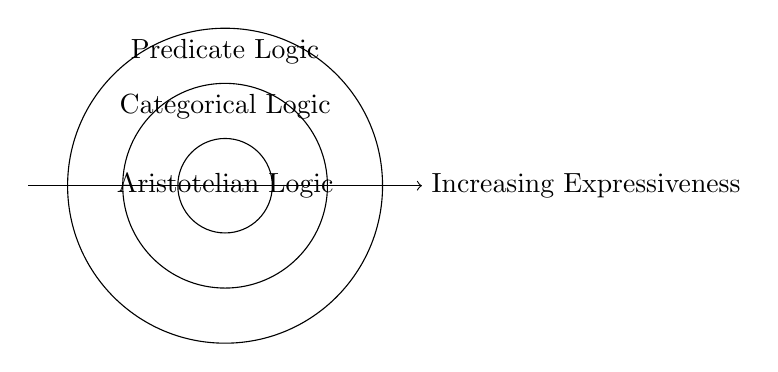
\begin{tikzpicture}
				\draw (0,0) circle (2cm);
				\draw (0,0) circle (1.3cm);
				\draw (0,0) circle (0.6cm);
				\node at (0,0) {Aristotelian Logic};
				\node at (0,1) {Categorical Logic};
				\node at (0,1.7) {Predicate Logic};
				\draw[->] (-2.5,0) -- (2.5,0) node[right] {Increasing Expressiveness};
			\end{tikzpicture}
		\end{center}
	\end{frame}
	
	\begin{frame}{Categorical Logic in Everyday Critical Thinking}

		\begin{itemize}
			\item Despite its limitations, categorical logic remains valuable for analyzing many common arguments.
			\item Understanding the patterns of valid categorical reasoning helps identify fallacies in everyday discourse.
			\item Categorical logic teaches the essential skill of determining when conclusions necessarily follow from premises.
			\item The principles of categorical logic form a foundation for more sophisticated critical thinking skills.
		\end{itemize}
		
		\begin{example}
			\scriptsize
			Political Argument: "No effective policies harm economic growth. This tax plan will harm economic growth. Therefore, this tax plan is not an effective policy."
			
			This can be analyzed as a categorical syllogism:\\
			No effective policies are things that harm economic growth. (E)\\
			This tax plan is a thing that harms economic growth. (A)\\
			Therefore, this tax plan is not an effective policy. (E)
			
			This is an EAE syllogism in the second figure, a valid form known as "Camestres."
		\end{example}
	\end{frame}
\end{document}